\documentclass[a4paper,12pt,twoside]{book}
\usepackage{lesi/lesi}

\title{Desenvolvimento de App WaVe Rotas Turísticas}
\author{Rui Jorge da Ponte Neiva}
\nrAluno{14103}
\regimeDiurno         % ou \regimePosLaboral
\LESI
\date{2020/2021}

%% Caso tenham mais que um orientador, colocar
%% \orientador{Nome professor \AND Nome professor}
\orientador{Maria Manuela Cruz da Cunha}

%% comentar estas três linhas para projectos
\empresa{Wave Solutions - Sistemas de Informação}
\enderecoEmpresa{Rua do Parque Industrial 5, 4755-539 Várzea}
\supervisor{Filipe Fonseca}

% comentar se não for para usar glossários
\makeglossaries




\begin{document}
\frontmatter
\maketitle  % print the title


\begin{resumo}
 
Resumo do trabalho realizado. Deve ser sucinto, e cobrir todo o relatório: uma introdução ao problema que se pretendeu resolver, um pequeno resumo da abordagem realizada, e algumas conclusões do trabalho atingido.

Poderão ser criados vários parágrafos, até para que cada um corresponda às três fases de introdução, desenvolvimento e conclusão.

Não é relevante colocar no resumo o local de estágio ou a referência ao curso. Essa informação já consta da capa.
\end{resumo}

\begin{abstract}
This is the translation of the previous text. It should say the exact same thing. Please do not use directly Google Translator.
\end{abstract}

%% Comment the following part if you are not acknowledging anybody
\begin{agradecimentos}
[A secção de agradecimentos é a parte pessoal do documento, e o único sítio onde o aluno pode escrever de forma menos formal, usando o tipo de linguagem que lhe parecer adequado para as pessoas a quem agradece.]
\end{agradecimentos}


\tableofcontents

% comentar se nao tiver figuraIs
\listoffigures

% comentar se nao tiver tabelas
\listoftables

% comentar se nao se quiser lista de listagens
\lstlistoflistings

% Commentar proximas duas linhas se nao for para usar acronimos




 \newacronym{ftp}{FTP}{File Transfer Protocol (Protocolo de Transferência de Ficheiros) }
 
 \newacronym{tcp}{TCP}{Transmission Control Protocol}
 
 \newacronym{http}{HTTP}{HyperText Transfer Protocol (Protocolo de Transferência de Hipertexto)}
\printglossary[type=\acronymtype,title={Siglas \& Acrónimos}]

% Commentar proximas duas linhas se nao for para usar glossarios



 \newglossaryentry{lematizador}
 {  
    name=lematizador,
    description={Com semelhanças com o Stemmer, também reduz uma palavra ao seu lema, que corresponde ao verbo no infinitivo no caso dos verbos, e ao masculino singular, no caso de nomes ou adjetivos. }
 }
 
\newglossaryentry{stemmer} 
{
    name=stemmer,
    description={Ferramenta capaz de reduzir uma palavra à sua raiz. Por exemplo, para a palavra ``correria'', a sua raiz seria ``corre''. }
 }
 

\printglossary


\printglossary


\mainmatter


\chapter{Introdução}

 [A introdução deve, tal como o próprio nome indica, introduzir o tema do trabalho. Não deve haver pressa em falar da empresa onde foi realizado o estágio ou o curso a que se refere o trabalho. Deve fazer-se uma introdução à área, Os Sistemas Informáticos ou as Ciências da Computação são áreas bastante grandes, pelo que não se deve supor que o leitor está a par das necessidades ou das tecnologias usadas em determinada área. No entanto, não devem ser explicados conceitos básicos, que qualquer licenciado numa engenharia de sistemas informáticos ou em ciências da computação tenham obrigação de conhecer.

 Na formatação do texto tente-se que não existam demasiadas zonas em branco. Não é pelo número de páginas que se mede a qualidade de um relatório. E, uma vez que os documentos são impressos, poupar algumas folhas é económico e ecológico. 

 Relembra-se que todo o conteúdo do documento deve ser original. Quaisquer citações retiradas de algum livro ou sítio da Internet devem ser devidamente formatadas, e a referência bibliográfica adicionada \citep{knuth1973}:
 
 \emph{By understanding a machine-oriented language, the programmer will tend to use a much more efficient method; it is much closer to reality. }

 Do mesmo modo, se algum texto, embora usando palavras do autor do documento, refira alguma ideia defendida por um outro autor, num outro documento, então também deverá aparecer a respetiva referência bibliográfica (PennState University Libraries, 2017). 
 
 

 O uso de citações é especialmente útil para defender ideias que outros autores também defendem, e que o autor do documento não tem com provar.] 

\section{Objetivos}
[Numa pequena secção da introdução liste, cuidadosamente, os objetivos do trabalho. Não confundir com os requisitos do software. Apenas o que se pretendia atingir originalmente.] 
\section{Contexto}
 [No caso de um estágio, é nesta secção que se deverá falar da empresa em que o estágio foi realizado. Se o projeto desenvolvido faz parte de um projeto mais amplo, faz sentido que se documente os objetivos do projeto com um todo, de modo que o leitor consiga perceber onde o trabalho realizado encaixa.] 
\section{Estrutura do documento}
 [A última secção da introdução deve explicar a estrutura do documento: quais são só capítulos existentes (para além do primeiro) e o que será discutido em cada um desses capítulos. A estrutura típica de um relatório de desenvolvimento de software é: 

 Introdução, com um breve resumo do que se pretende atingir, e uma descrição clara dos objetivos;

\begin{enumerate}
    \item Análise ao problema, que poderá incluir uma análise ao estado da arte ou ao modelo de negócio onde se pretende intervir;
    \item Análise e modelação do sistema, em que sejam levantados sistematicamente os requisitos, descritos diagramas de caso de uso e de atividade (que descrevam/formalizem o modelo de negócio). 
    \item Implementação, em que se descrevam as tecnologias escolhidas (e se justifiquem), e se refira detalhes sobre a implementação.
    \item Análise de resultados e testes, seja uma análise/avaliação aos resultados obtidos, sejam testes de usabilidade ou unitários ao trabalho desenvolvido. 
    \item Conclusão.]
\end{enumerate}{}


\chapter{Capitulo 2}

Este capítulo fala de \gls{stemmer}s. Mas não esquecer os \Gls{lematizador}es

\section{Sub-capitulo 1}

O \acrfull{http} é um protocolo baseado em \acrshort{tcp}.

\section{Figuras}

Ao contrário do Word, o \LaTeX{} usa um mecanismo de colocação de figuras e tabelas em que estas
flutuam ao longo das páginas de acordo com a necessidade/disponibilidade em termo de espaço vertical.
Assim, não devem usar frases como ``na figura acima'', ou ``na figura abaixo'', mas fazer referências:
``tal como se pode observar na Figura~\ref{fig:1}.''

\begin{figure}[htb]
    \centering
    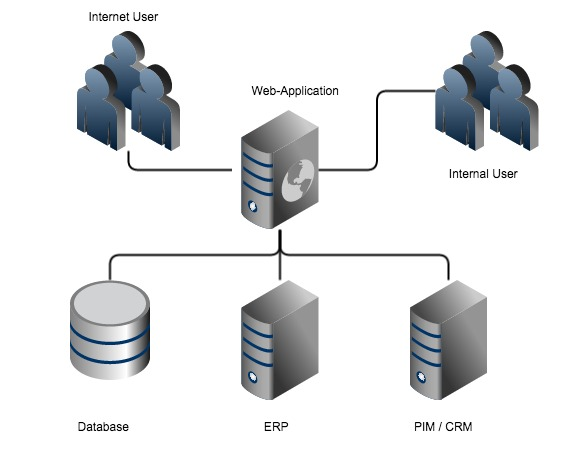
\includegraphics[width=0.8\linewidth]{images/sample}  % largura percentual 
    \caption{Esta é a legenda da figura}
    \label{fig:1}
\end{figure}

O mesmo acontece com as tabelas, como se pode ver na Tabela~\ref{tab:1}.

\begin{table}[htb]
    \centering
    \begin{tabular}{ccccc}
        \toprule
        \textbf{A} & \textbf{B} & \textbf{C} & \textbf{D} & \textbf{Total} \\
        \midrule
          1 & 2 & 3 & 4 & 10  \\
          2 & 3 & 4 & 5 & 14  \\
          3 & 4 & 5 & 6 & 18  \\
          4 & 5 & 6 & 7 & 22  \\
         \bottomrule
    \end{tabular}
    \caption{Legenda da tabela.}
    \label{tab:1}
\end{table}

Para a inclusão de código, usa-se algo semelhante. Veja-se a Listagem~\ref{lst:1}.

\begin{lstlisting}[language={[sharp]c},
                   caption={Método para contar o número de elementos numa lista iguais a uma determinada string.},
                   label=lst:1]
   public int count(string x) {
       return items.Select( y => y == x ).Count();
   }
\end{lstlisting}



\chapter{Capitulo 3}
\section{Sub-capitulo 1}
Texto do sub-capitulo 1
\section{Sub-capitulo 2}
Texto do sub-capitulo 2

\chapter{Capitulo 4}
\section{Sub-capitulo 1}
Texto do sub-capitulo 1
\section{Sub-capitulo 2}
Texto do sub-capitulo 2


\bibliography{biblio}

\end{document}
